\subsection{Experimentación:}

Se realizaron experimentos con instancias aleatorias, generadas utilizando la función rand()\footnote{http://www.cplusplus.com/reference/cstdlib/rand/}  perteneciente a la Standard Library.

Los experimentos se ejecutaron varias veces, para instancias diferentes, contando la cantidad de ciclos que conlleva resolver el problema y luego se promediaron los datos obtenidos.

\begin{center}
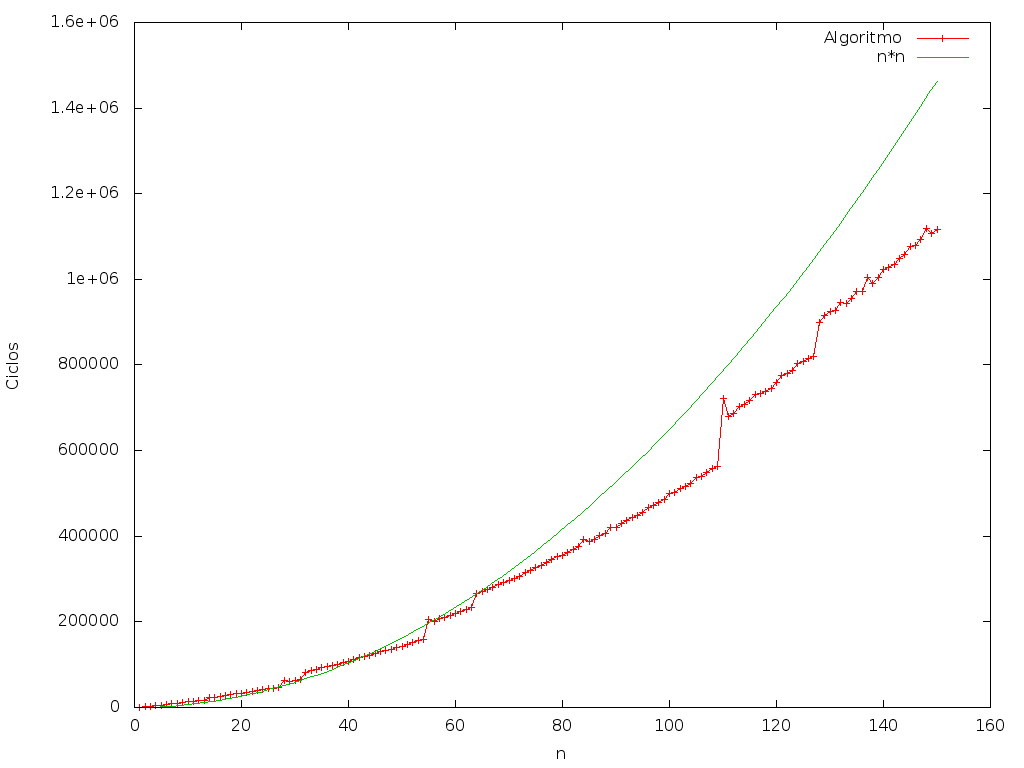
\includegraphics[scale=0.4]{../graficador/graficoAleatoriosEj1.png} 
\end{center}

Dada la naturaleza del algoritmo, no existe un peor caso. Ya que siempre debe llenar una matriz $n^{2}$ y buscar el mínimo dentro de la última columna.\\

Conclusiones:
\begin{itemize}
\item La cota calculada teóricamente era correcta.
\item La técnica de programación dinámica es muy efectiva en ciertos casos.
\end{itemize}